\documentclass[10pt]{article}
\usepackage{amsmath} 
\usepackage{graphicx}

\graphicspath{{../figs/}}

\begin{document}

\title{Guía 4 - Simulaciones de Monte Carlo}

\maketitle

\textbf{Problema 1: Susceptibilidad y fluctuaciones}
\\

Considere un sistema de spines discretos $S_i$ definidos en una red de $N$ sitios en presencia de un campo $B$, descripto por el Hamiltoniano $H$. Sea

\begin{equation}
m \equiv \dfrac{1}{N} \sum_i S_i,
\end{equation}

muestre las siguientes relaciones

\begin{align}
\chi &= \dfrac{\partial \langle m \rangle}{\partial B} = \beta N \left[ \langle m^2 \rangle - \langle m \rangle^2 \right],\\
C &= -T \dfrac{\partial^2 f(T,B)}{\partial T^2} = \dfrac{\beta^2}{N} \left[ \langle H^2 \rangle - \langle H \rangle^2 \right].
\end{align}


\textbf{Problema 2: Modelo de Ising en $d = 2$.}
\\

Considere el modelo de Ising en la red cuadrada de $L \times L$ sitios (parámetro de red unitario) con interacciones entre primeros vecinos:

\begin{equation}
H = - J \sum_{\langle i,j\rangle} S_i S_j - B \sum_i S_i.
\end{equation}

Usando condiciones de contorno periódicas y tomando la energía en unidades de $k_B$ (esto es, tomando $k_B = 1$) implemente un programa para simular las propiedades termodinámicas del modelo usando el algoritmo de Metropolis. Mediante este programa realice los siguientes cálculos:

\begin{itemize}

\item A campo nulo calcule las curvas de magnetización ($\langle |m| \rangle_L$), susceptibilidad y calor específico en función de $T/J$, para tamaños $L = 16, 32, 64, 128, \text{ y } 200$. Para cada magnitud grafique simultaneamente las curvas correspondientes a los diferentes tamaños. En el caso de la magnetización y el calor específico grafique también la solución exacta para la red infinita. Calcule en las mismas simulaciones las cantidades $\langle m^2 \rangle_L$ y $\langle m^4 \rangle_L$. Recuerde qeu cerca de la temperatura crítica los tiempos de relajación al equilibrio aumentan. Realice algunos tests preliminares.


\end{itemize}

\begin{figure}
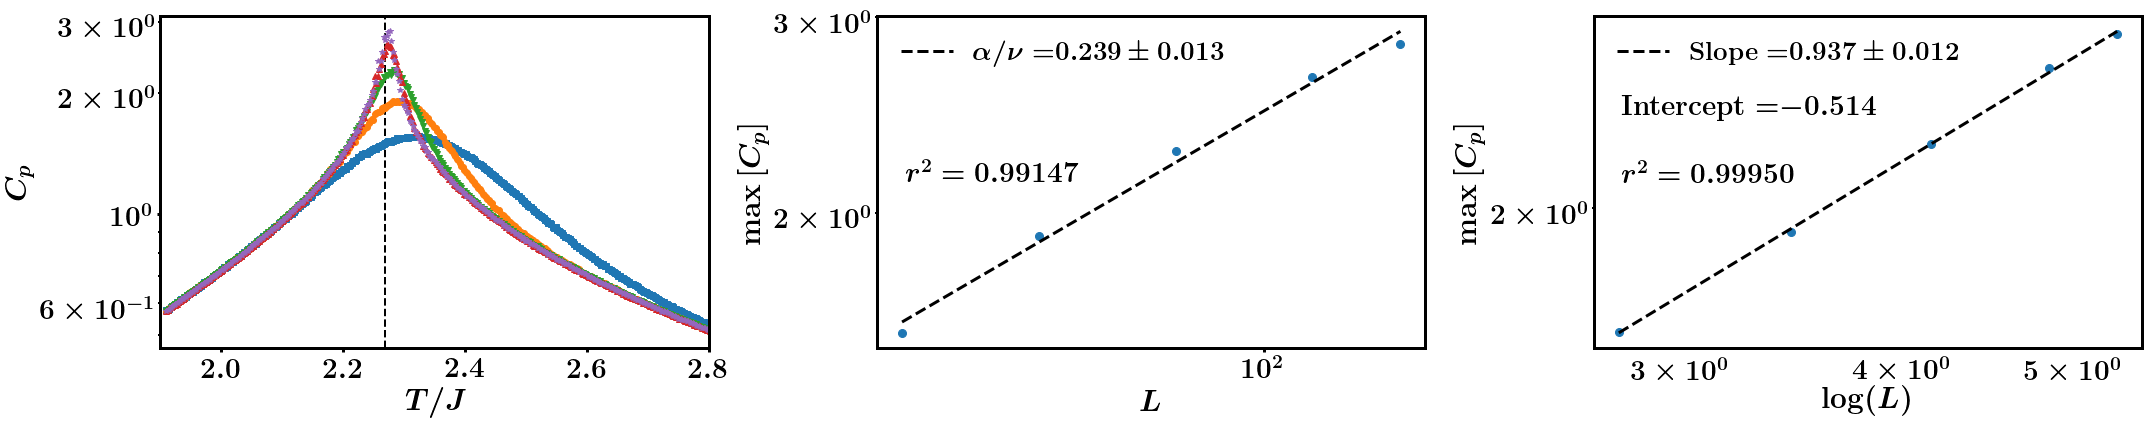
\includegraphics[scale=0.3]{Cp.png}
\end{figure}

\end{document}
